\chapter{Predictions}

All we did so far is predict what we already knew - the tale type of each text. We had the right answers already in our ATU Topic column. But what if we don't have this information? Could we perhaps predict tale types for unlabelled texts?

Open a new \widget{Corpus} widget and load the \emph{andersen.tab} corpus. Here we have three tales from H. C. Andersen. Inspect them in \widget{Corpus Viewer} and try to guess the tale type yourself.

\vspace{-0.2cm}
\begin{figure*}[h]
  \centering
  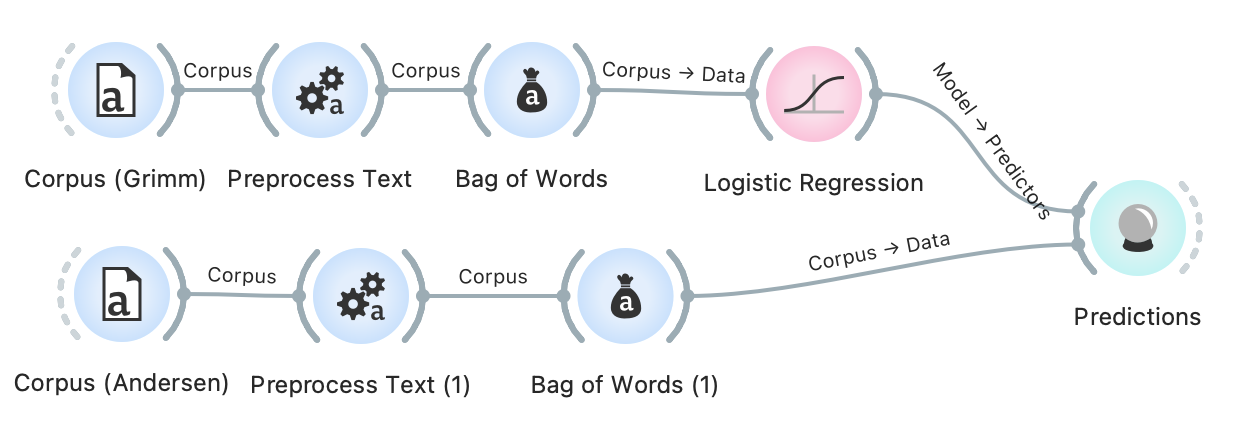
\includegraphics[width=0.8\linewidth]{workflow.png}%
  \caption{$\;$}
\end{figure*}
\vspace{-0.3cm}

Now connect them to \widget{Predictions} the same way as before - with \widget{Logistic Regression} passing the constructed model and the new Corpus widget passing the data for prediction. Do not forget to copy-paste the preprocessing widgets, namely \widget{Preprocess Text} and \widget{Bag of Words} to repeat data preparation.

Logistic Regression predicted all the tales to be Tales of Magic.\marginnote{Hint: Think about what kind of data the model was trained on and what were the most important words for the model.} The Ugly Duckling as a Tale of Magic? Sounds strange! Why do you think this happens?

\vspace{-0.2cm}
\begin{figure*}[h]
  \centering
  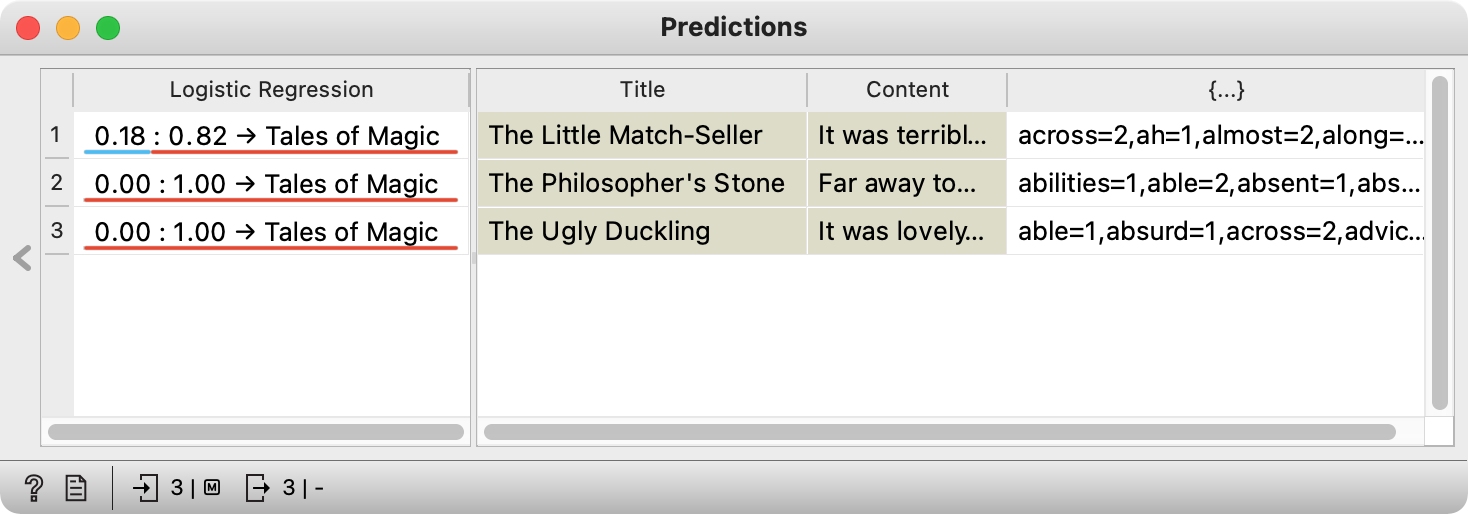
\includegraphics[width=\linewidth]{predictions.png}%
  \caption{$\;$}
\end{figure*}
\vspace{-0.3cm}
